\documentclass[]{article}
\usepackage{lmodern}
\usepackage{amssymb,amsmath}
\usepackage{ifxetex,ifluatex}
\usepackage{fixltx2e} % provides \textsubscript
\ifnum 0\ifxetex 1\fi\ifluatex 1\fi=0 % if pdftex
  \usepackage[T1]{fontenc}
  \usepackage[utf8]{inputenc}
\else % if luatex or xelatex
  \ifxetex
    \usepackage{mathspec}
  \else
    \usepackage{fontspec}
  \fi
  \defaultfontfeatures{Ligatures=TeX,Scale=MatchLowercase}
\fi
% use upquote if available, for straight quotes in verbatim environments
\IfFileExists{upquote.sty}{\usepackage{upquote}}{}
% use microtype if available
\IfFileExists{microtype.sty}{%
\usepackage{microtype}
\UseMicrotypeSet[protrusion]{basicmath} % disable protrusion for tt fonts
}{}
\usepackage[margin=1in]{geometry}
\usepackage{hyperref}
\hypersetup{unicode=true,
            pdftitle={SEM 1},
            pdfauthor={Simon Roth},
            pdfborder={0 0 0},
            breaklinks=true}
\urlstyle{same}  % don't use monospace font for urls
\usepackage{graphicx,grffile}
\makeatletter
\def\maxwidth{\ifdim\Gin@nat@width>\linewidth\linewidth\else\Gin@nat@width\fi}
\def\maxheight{\ifdim\Gin@nat@height>\textheight\textheight\else\Gin@nat@height\fi}
\makeatother
% Scale images if necessary, so that they will not overflow the page
% margins by default, and it is still possible to overwrite the defaults
% using explicit options in \includegraphics[width, height, ...]{}
\setkeys{Gin}{width=\maxwidth,height=\maxheight,keepaspectratio}
\IfFileExists{parskip.sty}{%
\usepackage{parskip}
}{% else
\setlength{\parindent}{0pt}
\setlength{\parskip}{6pt plus 2pt minus 1pt}
}
\setlength{\emergencystretch}{3em}  % prevent overfull lines
\providecommand{\tightlist}{%
  \setlength{\itemsep}{0pt}\setlength{\parskip}{0pt}}
\setcounter{secnumdepth}{5}
% Redefines (sub)paragraphs to behave more like sections
\ifx\paragraph\undefined\else
\let\oldparagraph\paragraph
\renewcommand{\paragraph}[1]{\oldparagraph{#1}\mbox{}}
\fi
\ifx\subparagraph\undefined\else
\let\oldsubparagraph\subparagraph
\renewcommand{\subparagraph}[1]{\oldsubparagraph{#1}\mbox{}}
\fi

%%% Use protect on footnotes to avoid problems with footnotes in titles
\let\rmarkdownfootnote\footnote%
\def\footnote{\protect\rmarkdownfootnote}

%%% Change title format to be more compact
\usepackage{titling}

% Create subtitle command for use in maketitle
\newcommand{\subtitle}[1]{
  \posttitle{
    \begin{center}\large#1\end{center}
    }
}

\setlength{\droptitle}{-2em}
  \title{SEM 1}
  \pretitle{\vspace{\droptitle}\centering\huge}
  \posttitle{\par}
  \author{Simon Roth}
  \preauthor{\centering\large\emph}
  \postauthor{\par}
  \predate{\centering\large\emph}
  \postdate{\par}
  \date{19.4.2017}

\usepackage{pdflscape}
\newcommand{\blandscape}{\begin{landscape}}
\newcommand{\elandscape}{\end{landscape}}
\usepackage{rotating}

\begin{document}
\maketitle

{
\setcounter{tocdepth}{2}
\tableofcontents
}
\section{Datensatz einladen}\label{datensatz-einladen}

\begin{enumerate}
\def\labelenumi{\alph{enumi}.}
\tightlist
\item
  german: Staatsbürgerschaft
\end{enumerate}

\begin{itemize}
\tightlist
\item
  1 Ja, ausschließlich
\item
  2 Ja, neben 2. Staatsbürgerschaft
\item
  3 Nein
\end{itemize}

\begin{enumerate}
\def\labelenumi{\alph{enumi}.}
\setcounter{enumi}{1}
\tightlist
\item
  eastwest: Erhebungsgebiet
\end{enumerate}

\begin{itemize}
\tightlist
\item
  1 West
\item
  2 Ost
\end{itemize}

\subsection{Itembatterien}\label{itembatterien}

\textbf{Islamophobie:}

\begin{itemize}
\tightlist
\item
  mm01: ISLAMAUSUEBUNG IN BRD BESCHRAENKEN

  \begin{itemize}
  \tightlist
  \item
    -10 Befragter gehört einer islamischen Religionsgemeinschaft an
    (Code 1 in rd03)
  \item
    -9
  \item
    1 Stimme überhaupt nicht zu
  \item
    2
  \item
    3
  \item
    4
  \item
    5
  \item
    6
  \item
    7 Stimme voll und ganz zu
  \end{itemize}
\item
  mm02: ISLAM PASST IN DIE DEUTSCHE GESELLSCHAFT
\item
  mm03: ANWESENHEIT VON MUSLIMEN BRINGT KONFLIKT
\item
  mm04: STAAT SOLLTE ISLAM. GRUPPEN BEOBACHTEN
\item
  mm05: MUSLIMISCHER BUERGERMEISTER IN ORDNUNG
\item
  mm06: UNTER MUSLIMEN SIND VIELE REL. FANATIKER
\end{itemize}

\textbf{Deutschein:}

\begin{itemize}
\tightlist
\item
  mn11: DEUTSCH SEIN: DEUTSCHE STAATSBUERGERSCH.
\item
  mn12: DEUTSCH SEIN: CHRISTL.RELIGION ZUGEHOER.
\item
  mn13: DEUTSCH SEIN: BEKENNTNIS ZUR DEMOKRATIE
\item
  mn14: DEUTSCH SEIN: VIELE DEUTSCHE BEKANNTE
\item
  mn15: DEUTSCH SEIN: ALTE STAATSANGEH.AUFGEBEN
\item
  mn16: DEUTSCH SEIN: VERBUNDENHEIT ZU DEUTSCHL.
\item
  mn17: DEUTSCH SEIN: ALTE GEBRAEUCHE ABLEGEN
\item
  mn18: DEUTSCH SEIN: GUT DEUTSCH SPRECHEN
\item
  mn19: DEUTSCH SEIN: WESTLICHE WERTE TEILEN
\item
  mn20: DEUTSCH SEIN: MIND. 1 ELTERNTEIL DEUTSCH
\item
  mn21: DEUTSCH SEIN: IN DEUTSCHLAND GEBOREN
\end{itemize}

\section{Daten partitionieren}\label{daten-partitionieren}

\begin{itemize}
\tightlist
\item
  sex: GESCHLECHT (Int.: Geschlecht der befragten Person ohne Befragen
  eintragen!)

  \begin{itemize}
  \tightlist
  \item
    1 Männlich
  \item
    2 Weiblich
  \end{itemize}
\item
  age: ALTER: metrisch
\item
  agec: ALTER: KATEGORISIERT 6

  \begin{itemize}
  \tightlist
  \item
    18 - 29 Jahre
  \item
    30 - 44 Jahre
  \item
    45 - 59 Jahre
  \item
    60 - 74 Jahre
  \item
    75 - 89 Jahre
  \item
    Über 89 Jahre
  \end{itemize}
\item
  isced97: BEFR.: ISCED 1997 - 6 STUFEN: International Standard
  Classification of Education (ISCED) 1997, 6 Stufen

  \begin{enumerate}
  \def\labelenumi{\arabic{enumi}.}
  \tightlist
  \item
    Level - Primary education or first stage of basic education
  \item
    Level - Lower secondary or second stage of basic education
  \item
    Level - (Upper) secondary education
  \item
    Level - Post-secondary non-tertiary education
  \item
    Level - First stage of tertiary education
  \item
    Level - Second stage of tertiary education
  \end{enumerate}
\end{itemize}

\section{Visualisierungen}\label{visualisierungen}

\begin{center}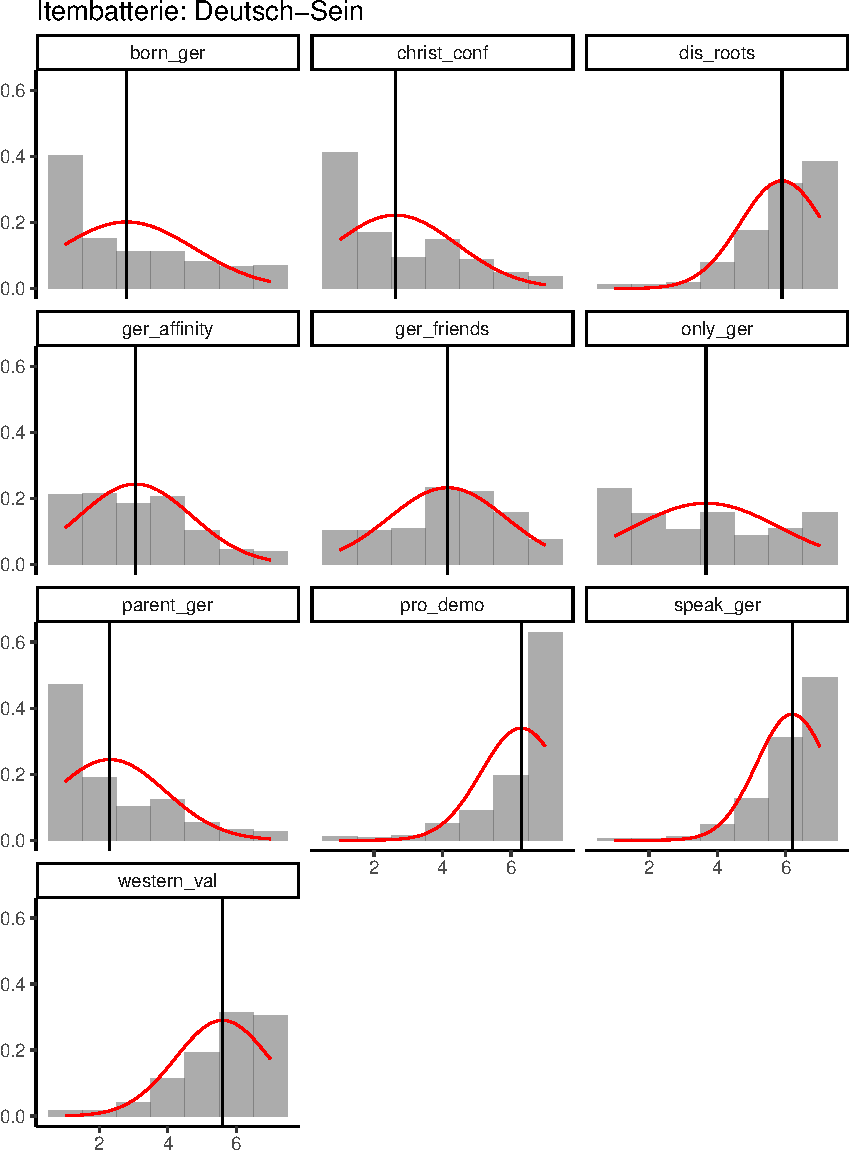
\includegraphics{session_1_files/figure-latex/vis-1} \end{center}

\begin{center}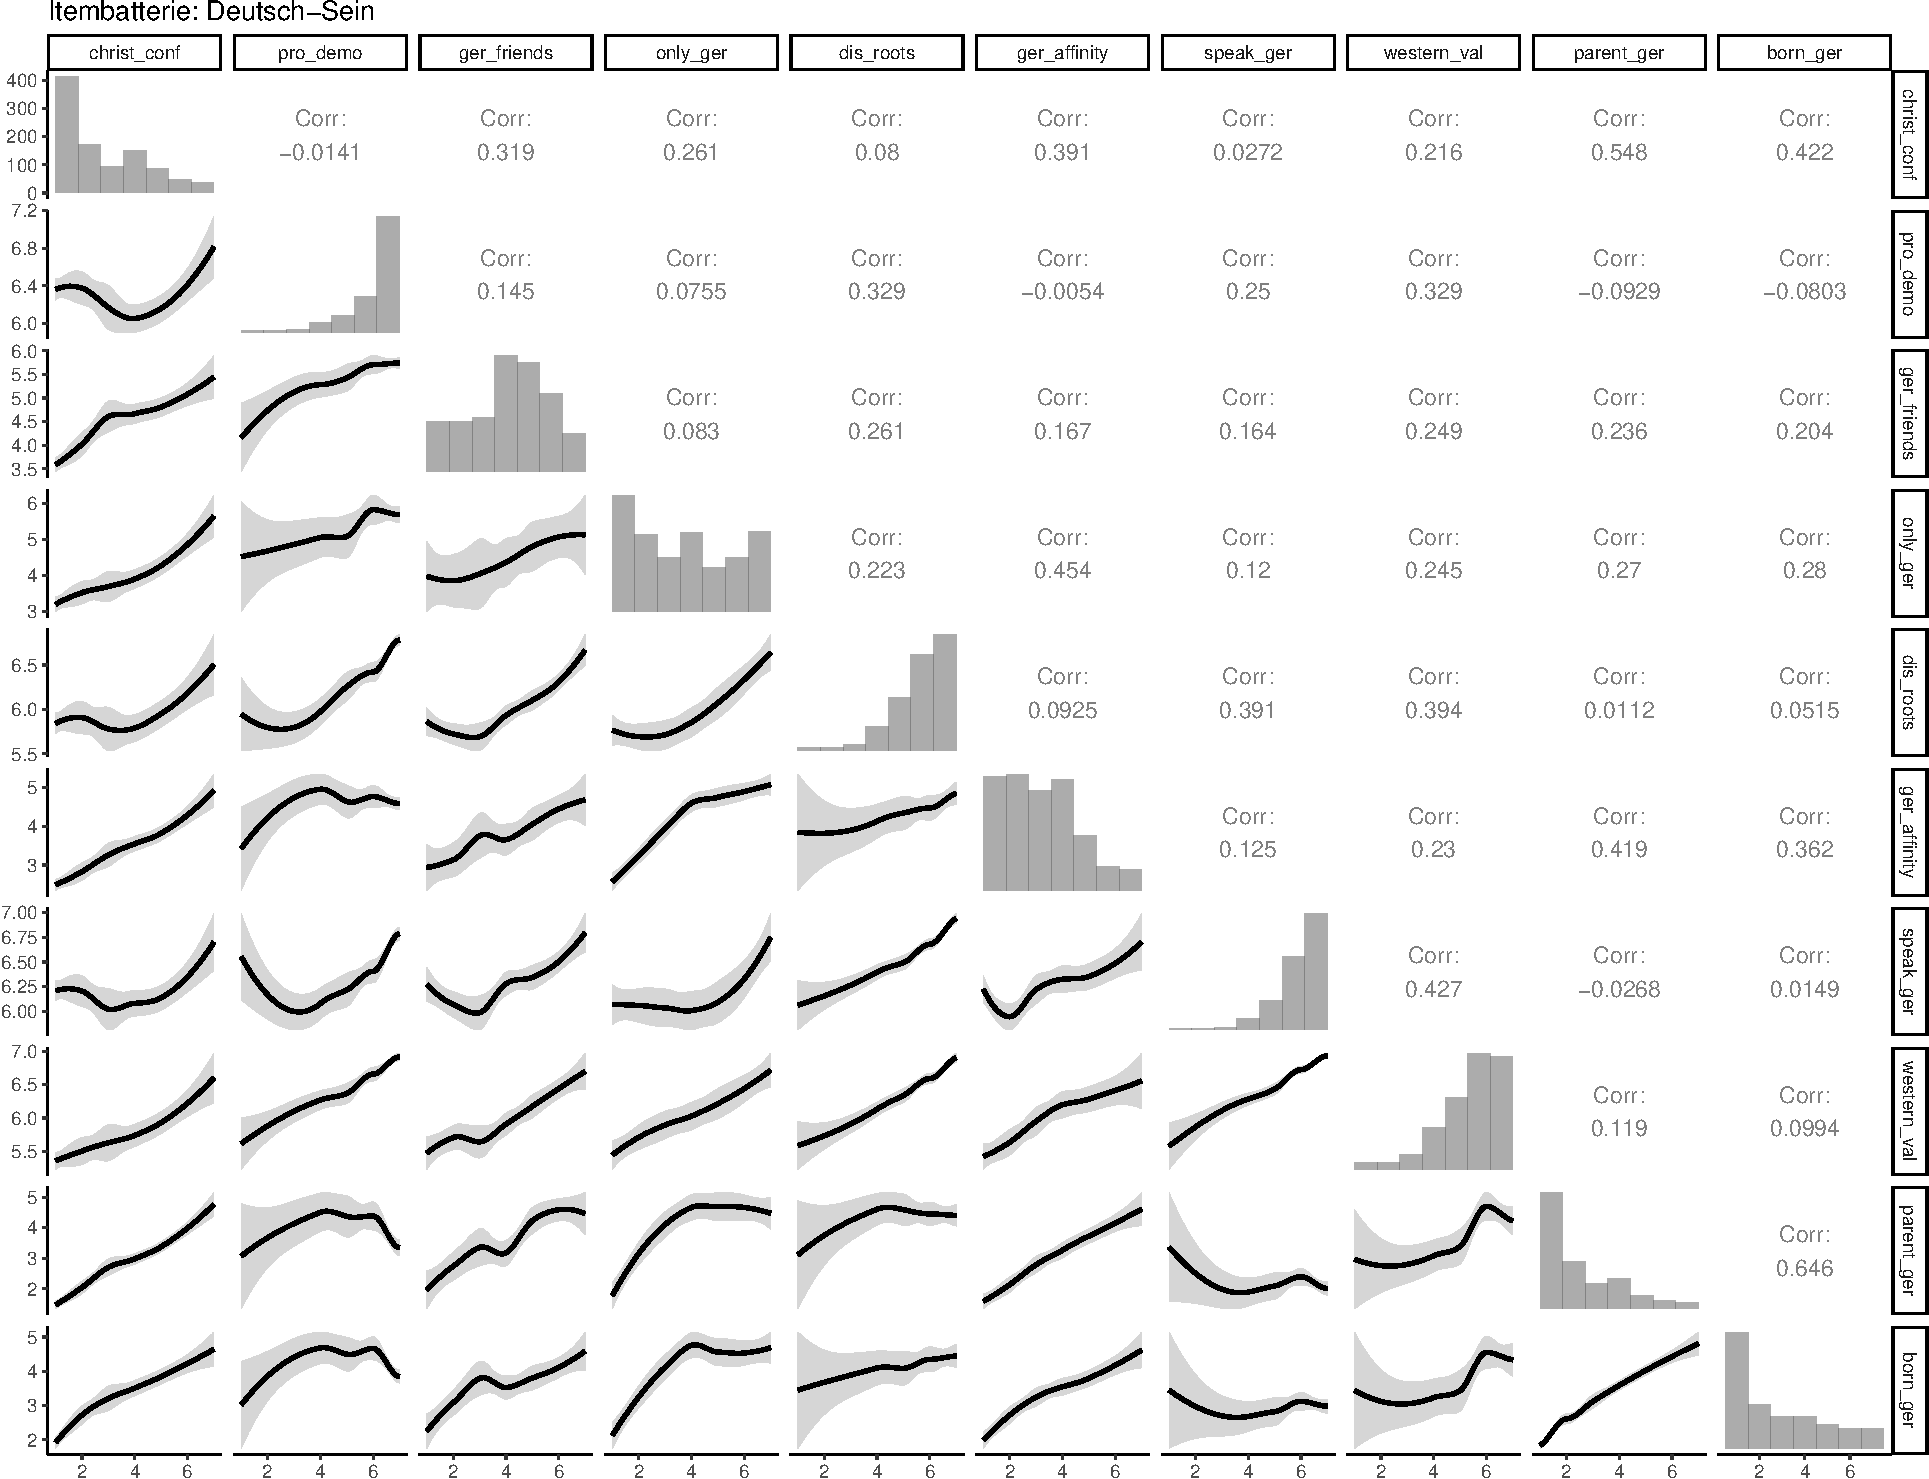
\includegraphics{session_1_files/figure-latex/unnamed-chunk-1-1} \end{center}

\newpage

\blandscape
Landscape

\begin{table}[ht]
\centering
\begingroup\small
\begin{tabular}{rrrrrrrrrrrrrrrrrrrr}
  \hline
 & \begin{sideways} age \end{sideways} & \begin{sideways} isced97 \end{sideways} & \begin{sideways} ger\_citiz \end{sideways} & \begin{sideways} christ\_conf \end{sideways} & \begin{sideways} pro\_demo \end{sideways} & \begin{sideways} ger\_friends \end{sideways} & \begin{sideways} only\_ger \end{sideways} & \begin{sideways} dis\_roots \end{sideways} & \begin{sideways} ger\_affinity \end{sideways} & \begin{sideways} speak\_ger \end{sideways} & \begin{sideways} western\_val \end{sideways} & \begin{sideways} parent\_ger \end{sideways} & \begin{sideways} born\_ger \end{sideways} & \begin{sideways} stop\_islam \end{sideways} & \begin{sideways} islam\_is\_ger \end{sideways} & \begin{sideways} muslim\_confl \end{sideways} & \begin{sideways} muslim\_surv \end{sideways} & \begin{sideways} muslim\_major \end{sideways} & \begin{sideways} muslim\_rad \end{sideways} \\ 
  \hline
age & 1.00 & 0.00 & 0.11 & 0.17 & 0.12 & 0.13 & 0.21 & 0.14 & 0.12 & 0.09 & 0.18 & 0.14 & 0.13 & 0.16 & -0.18 & 0.11 & 0.26 & -0.16 & 0.30 \\ 
  isced97 &  & 1.00 & -0.09 & -0.12 & 0.14 & 0.03 & -0.14 & 0.03 & -0.18 & -0.03 & -0.04 & -0.17 & -0.17 & -0.20 & 0.17 & -0.10 & -0.15 & 0.21 & -0.22 \\ 
  ger\_citiz &  &  & 1.00 & 0.19 & 0.29 & 0.10 & 0.36 & 0.27 & 0.20 & 0.22 & 0.30 & 0.12 & 0.18 & 0.13 & -0.15 & 0.18 & 0.18 & -0.11 & 0.17 \\ 
  christ\_conf &  &  &  & 1.00 & -0.01 & 0.32 & 0.26 & 0.08 & 0.39 & 0.03 & 0.22 & 0.55 & 0.42 & 0.38 & -0.27 & 0.24 & 0.32 & -0.32 & 0.33 \\ 
  pro\_demo &  &  &  &  & 1.00 & 0.15 & 0.08 & 0.33 & -0.01 & 0.25 & 0.33 & -0.09 & -0.08 & -0.05 & 0.06 & 0.06 & 0.06 & 0.06 & -0.01 \\ 
  ger\_friends &  &  &  &  &  & 1.00 & 0.08 & 0.26 & 0.17 & 0.16 & 0.25 & 0.24 & 0.20 & 0.09 & -0.00 & 0.14 & 0.16 & -0.07 & 0.10 \\ 
  only\_ger &  &  &  &  &  &  & 1.00 & 0.22 & 0.45 & 0.12 & 0.25 & 0.27 & 0.28 & 0.30 & -0.27 & 0.21 & 0.26 & -0.30 & 0.31 \\ 
  dis\_roots &  &  &  &  &  &  &  & 1.00 & 0.09 & 0.39 & 0.39 & 0.01 & 0.05 & 0.05 & 0.01 & 0.17 & 0.15 & -0.04 & 0.08 \\ 
  ger\_affinity &  &  &  &  &  &  &  &  & 1.00 & 0.12 & 0.23 & 0.42 & 0.36 & 0.43 & -0.32 & 0.26 & 0.31 & -0.38 & 0.36 \\ 
  speak\_ger &  &  &  &  &  &  &  &  &  & 1.00 & 0.43 & -0.03 & 0.01 & 0.08 & -0.10 & 0.17 & 0.16 & -0.05 & 0.16 \\ 
  western\_val &  &  &  &  &  &  &  &  &  &  & 1.00 & 0.12 & 0.10 & 0.20 & -0.18 & 0.20 & 0.26 & -0.17 & 0.23 \\ 
  parent\_ger &  &  &  &  &  &  &  &  &  &  &  & 1.00 & 0.65 & 0.33 & -0.23 & 0.23 & 0.28 & -0.28 & 0.30 \\ 
  born\_ger &  &  &  &  &  &  &  &  &  &  &  &  & 1.00 & 0.30 & -0.22 & 0.19 & 0.27 & -0.27 & 0.28 \\ 
  stop\_islam &  &  &  &  &  &  &  &  &  &  &  &  &  & 1.00 & -0.54 & 0.42 & 0.49 & -0.49 & 0.51 \\ 
  islam\_is\_ger &  &  &  &  &  &  &  &  &  &  &  &  &  &  & 1.00 & -0.36 & -0.42 & 0.50 & -0.42 \\ 
  muslim\_confl &  &  &  &  &  &  &  &  &  &  &  &  &  &  &  & 1.00 & 0.52 & -0.33 & 0.42 \\ 
  muslim\_surv &  &  &  &  &  &  &  &  &  &  &  &  &  &  &  &  & 1.00 & -0.42 & 0.52 \\ 
  muslim\_major &  &  &  &  &  &  &  &  &  &  &  &  &  &  &  &  &  & 1.00 & -0.44 \\ 
  muslim\_rad &  &  &  &  &  &  &  &  &  &  &  &  &  &  &  &  &  &  & 1.00 \\ 
   \hline
\end{tabular}
\endgroup
\caption{Pearson's correlation matrix} 
\end{table}

\elandscape

\subsection{Interactive}\label{interactive}

\subsection{Easy}\label{easy}

\newpage

\blandscape

\begin{center}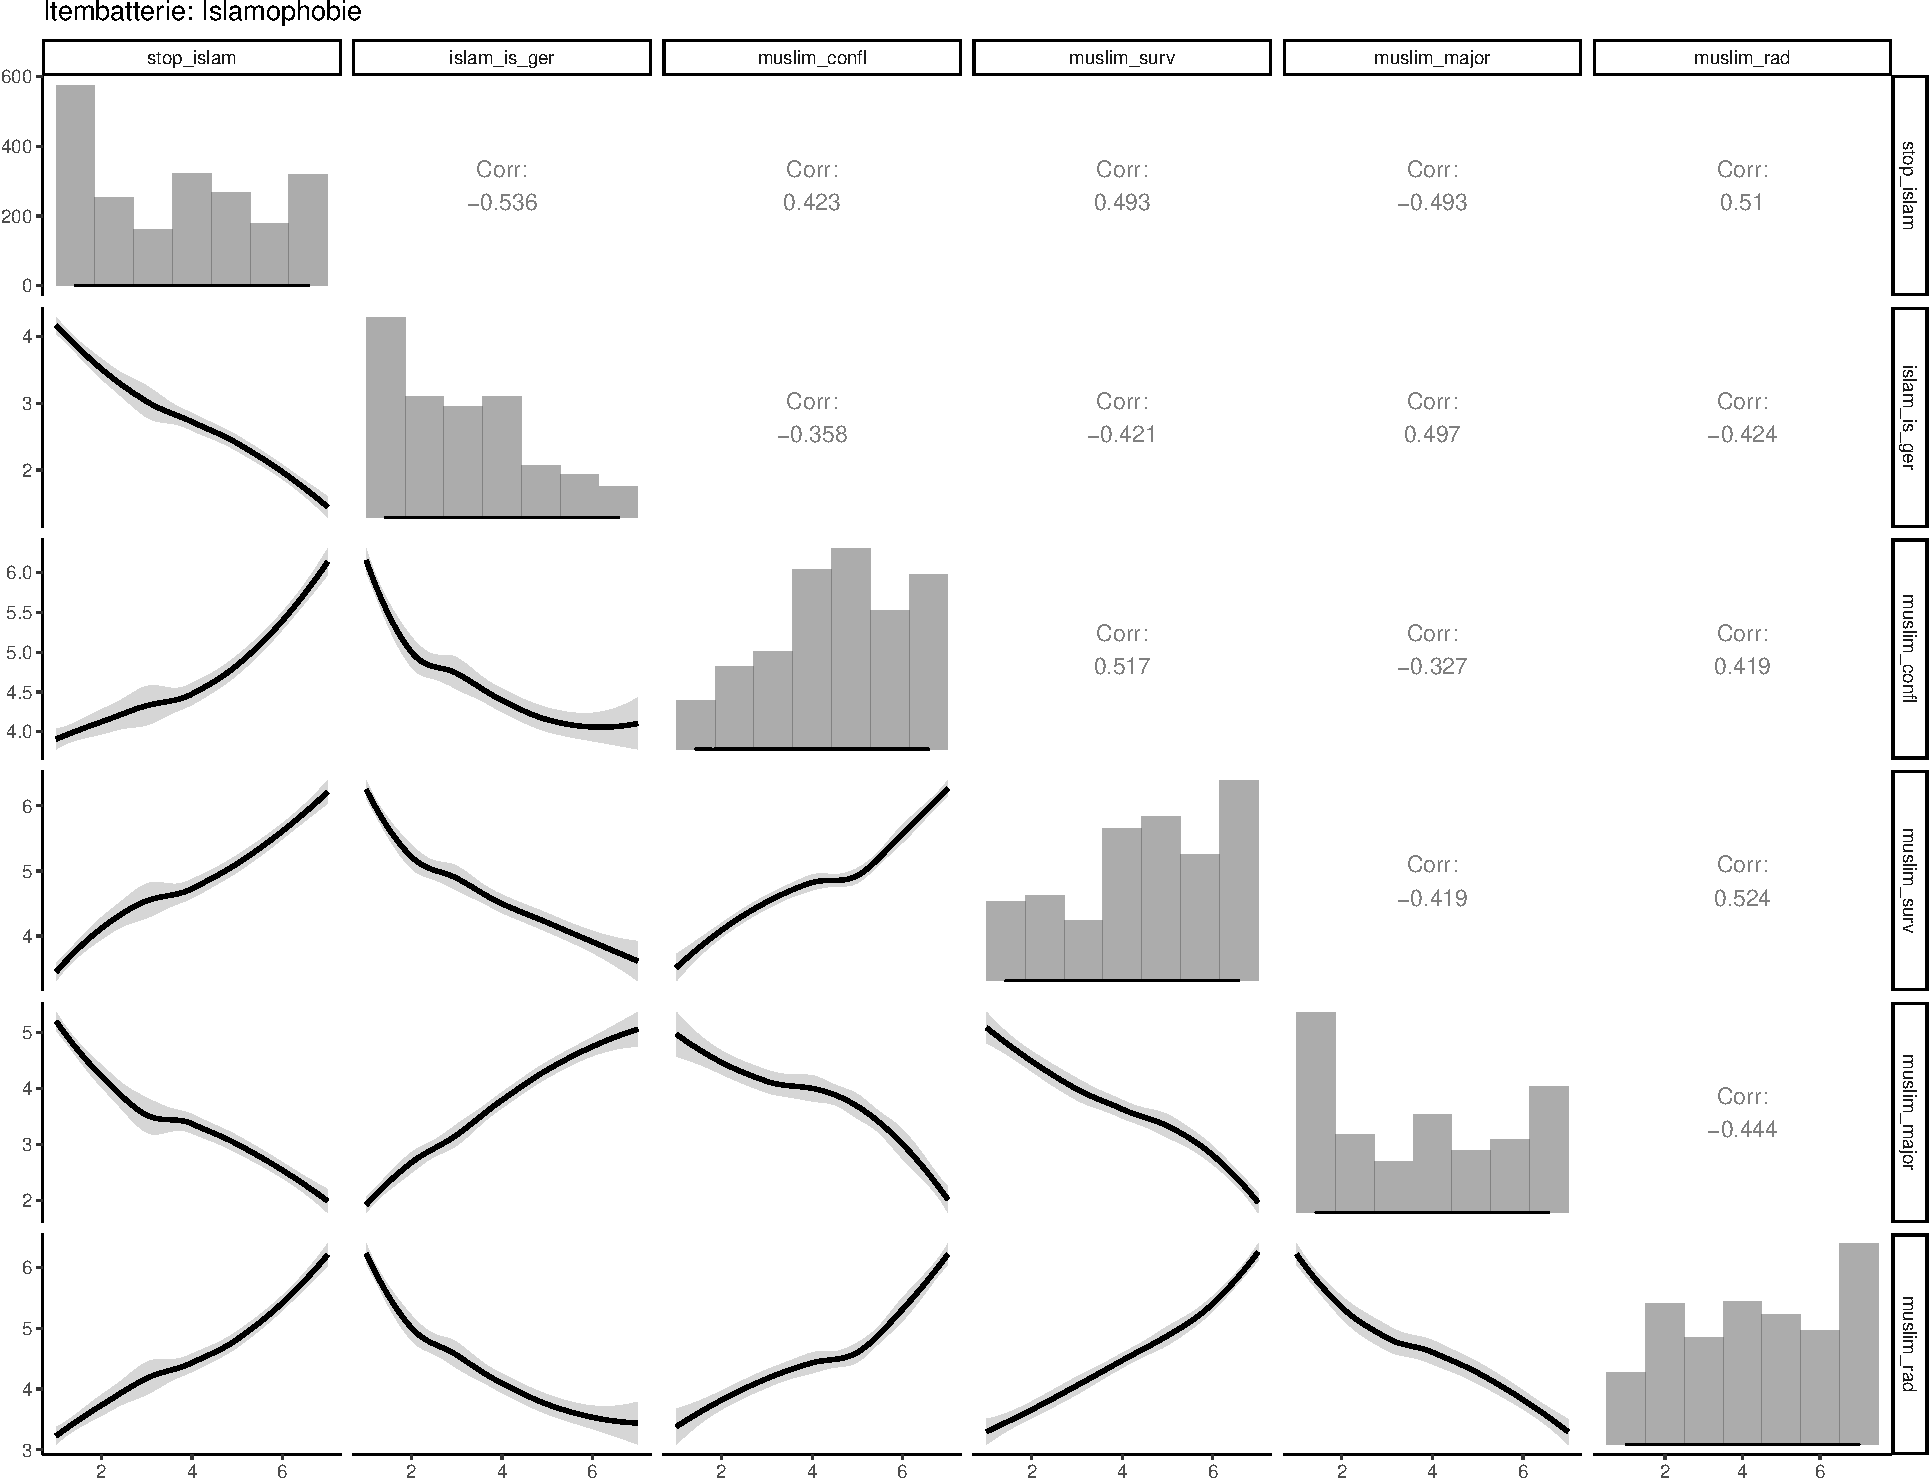
\includegraphics{session_1_files/figure-latex/unnamed-chunk-5-1} \end{center}

\elandscape


\end{document}
